\documentclass[UTF8,11pt]{ctexart}

\usepackage[a4paper,top=2.35cm,bottom=2.25cm,left=2.45cm,right=2.45cm,headheight=15pt]{geometry}
\usepackage{fontspec}
\setmainfont{TeX Gyre Pagella}
\setsansfont{TeX Gyre Heros}
\setmonofont{DejaVu Sans Mono}[Scale=0.84]
\setCJKmainfont{Noto Serif CJK SC}
\setCJKsansfont{Noto Sans CJK SC}
\setCJKmonofont{Noto Sans Mono CJK SC}

\usepackage{amsmath,amssymb,bm}
\usepackage{graphicx}
\usepackage{booktabs,tabularx,array,multirow,longtable}
\usepackage{siunitx}
\usepackage[dvipsnames]{xcolor}
\usepackage{tikz}
\usepackage[most]{tcolorbox}
\usepackage{enumitem}
\usepackage{caption}
\usepackage{float}
\usepackage{fancyhdr}
\usepackage{titlesec}
\usepackage{listings}
\usepackage{xurl}
\usepackage{hyperref}
\usepackage{lastpage}

\definecolor{Navy}{HTML}{153F66}
\definecolor{Blue}{HTML}{2F6F9F}
\definecolor{Teal}{HTML}{2A8C82}
\definecolor{Green}{HTML}{4D8F62}
\definecolor{Orange}{HTML}{D9822B}
\definecolor{LightBlue}{HTML}{EEF5FA}
\definecolor{LightGray}{HTML}{F4F6F8}
\definecolor{Dark}{HTML}{25313B}

\hypersetup{
  colorlinks=true,
  linkcolor=Navy,
  urlcolor=Blue,
  citecolor=Teal,
  pdftitle={基于改进型 Fourier Neural Operator 的深海声传播损失快速计算技术报告},
  pdfauthor={Ocean Acoustic Surrogate Project},
  pdfsubject={数据集构建、模型方法与实验结果}
}

\graphicspath{{assets/}{../assets/}}
\captionsetup{font=small,labelfont={bf,color=Navy}}
\setlist{leftmargin=2em,itemsep=0.2em,topsep=0.3em}
\renewcommand{\arraystretch}{1.25}
\setlength{\tabcolsep}{5pt}
\setcounter{tocdepth}{1}
\setcounter{secnumdepth}{3}

\titleformat{\section}{\LARGE\bfseries\sffamily\color{Navy}}{\thesection}{0.7em}{}
  [\vspace{0.2em}\color{Blue}\titlerule]
\titleformat{\subsection}{\Large\bfseries\sffamily\color{Navy}}{\thesubsection}{0.7em}{}
\titleformat{\subsubsection}{\large\bfseries\sffamily\color{Blue}}{\thesubsubsection}{0.6em}{}

\pagestyle{fancy}
\fancyhf{}
\fancyhead[L]{\small\sffamily\color{Navy}深海声传播损失快速计算}
\fancyhead[R]{\small\sffamily\color{Navy}项目技术报告 V1.2}
\fancyfoot[L]{\small\color{gray}Ocean Acoustic Surrogate Project}
\fancyfoot[R]{\small\color{gray}\thepage\,/\,\pageref{LastPage}}
\renewcommand{\headrulewidth}{0.45pt}
\renewcommand{\footrulewidth}{0pt}

\newcolumntype{Y}{>{\raggedright\arraybackslash}X}
\newcolumntype{C}[1]{>{\centering\arraybackslash}p{#1}}
\newcolumntype{L}[1]{>{\raggedright\arraybackslash}p{#1}}

\newtcolorbox{summarybox}{
  enhanced,
  breakable,
  colback=LightBlue,
  colframe=Blue,
  boxrule=0.7pt,
  arc=1mm,
  left=4mm,right=4mm,top=3mm,bottom=3mm
}

\lstdefinestyle{repro}{
  basicstyle=\ttfamily\footnotesize,
  backgroundcolor=\color{LightGray},
  frame=single,
  rulecolor=\color{gray!35},
  breaklines=true,
  columns=fullflexible,
  keepspaces=true,
  showstringspaces=false,
  xleftmargin=0.8em,
  framexleftmargin=0.6em,
  aboveskip=0.6em,
  belowskip=0.6em
}

\newcommand{\figfull}[3]{
  \begin{figure}[H]
    \centering
    \includegraphics[width=#1\textwidth]{#2}
    \caption{#3}
  \end{figure}
}
\newcommand{\TL}{\mathrm{TL}}
\newcommand{\RMSE}{\mathrm{RMSE}}

\begin{document}

% -----------------------------------------------------------------------------
% Title page
% -----------------------------------------------------------------------------
\begin{titlepage}
\begin{tikzpicture}[remember picture,overlay]
  \fill[Navy] (current page.north west) rectangle ([yshift=-1.4cm]current page.north east);
  \fill[Blue] ([yshift=-1.4cm]current page.north west) rectangle ([yshift=-1.52cm]current page.north east);
\end{tikzpicture}

\vspace*{2.0cm}
{\sffamily\color{Blue}\Large 项目技术报告}\par
\vspace{0.8cm}
{\sffamily\bfseries\color{Navy}\fontsize{27}{35}\selectfont
基于改进型 FNO 的\par
深海声传播损失快速计算}\par
\vspace{0.7cm}
{\sffamily\color{Dark}\Large
Fourier Neural Operator 方法、数据集构建与实验结果}\par

\vspace{1.6cm}
\begin{summarybox}
\centering
\begin{tabular}{L{3.4cm}L{7.8cm}}
\textbf{核心场景} & 1 kHz、50 km、2000 m 深海、50 m 声源深度 \\
\textbf{研究任务} & 从一维声速剖面快速预测二维非相干传播损失场 \\
\textbf{参考方法} & Bellhop，25,600 条射线/场 \\
\textbf{最终结果} & 测试 RMSE 0.5165 dB，A100 P95 4.73 ms \\
\textbf{报告版本} & V1.2，2026-08-27 \\
\end{tabular}
\end{summarybox}

\vfill
{\sffamily\color{Navy}\Large Ocean Acoustic Surrogate Project}\par
\vspace{0.3cm}
{\color{Dark}面向固定典型深海场景的声场快速代理计算研究}\par
\vspace{1.1cm}
\end{titlepage}

\pagenumbering{roman}

% -----------------------------------------------------------------------------
\section*{摘\quad 要}
\addcontentsline{toc}{section}{摘要}

针对传统声传播数值模型计算成本较高、难以直接支持在线快速评估的问题，本项目研究从
一维声速剖面（Sound Speed Profile, SSP）到二维传播损失（Transmission Loss, TL）场的
数据驱动代理计算方法。研究场景固定为频率 1 kHz、最大传播距离 50 km、水深 2000 m、
声源深度 50 m、距离无关的典型深海环境，输出为 96$\times$256 深度--距离网格上的
Bellhop 非相干 TL。

数据集以项目早期资料提供的\textbf{南海东侧海域 6 月仿真深海 SSP 形态}为原型。该原型
由 11 个深度--声速控制点表示，并通过全局声速偏移、上层温跃层强度、声道轴深度和
深层梯度四个具有明确物理含义的参数构造 512 条平滑 SSP。四维参数采用优化 Latin
hypercube 采样，幅度限制在典型深海剖面的窄变化范围内。由于本阶段目标场景为固定水深、
距离无关环境，因此未引入外部海底地形数据，也未混合多月份、多方位或跨海区剖面。

在标签生成方面，项目首先在 8 条独立 SSP 上进行 3,200--25,600 射线的逐级收敛实验，
随后固定采用每场 25,600 条射线生成 512 个 Bellhop 高质量参考声场。模型方面，在标准
Fourier Neural Operator（FNO）的基础上，针对深度--距离网格的强各向异性和非周期边界，
提出各向异性谱截断、复制填充、层间残差连接和训练均值场残差学习的组合方法。

在 384/64/64 的训练、验证和独立测试划分上，最终模型测试集 RMSE 为 0.5165 dB，MAE
为 0.1802 dB，最差单样本 RMSE 为 0.7687 dB；A100 GPU 上 batch=1 完整推理 P95 为
4.73 ms，均显著优于 RMSE 不超过 2 dB、推理时间不超过 100 ms 的目标指标。结果表明，
在给定的核心场景内，改进型 FNO 可以有效保留深海声场中的主要会聚结构，并实现相对于
Bellhop 约三个数量级的在线计算加速。

\vspace{0.6cm}
\noindent\textbf{关键词：}水声传播；传播损失；Bellhop；Fourier Neural Operator；代理模型；深海声速剖面

\clearpage
\tableofcontents
\clearpage
\pagenumbering{arabic}

% -----------------------------------------------------------------------------
\section{研究背景与任务定义}

\subsection{研究背景}

深海声传播受到声速随深度变化、海面与海底边界以及多路径会聚效应的共同影响。Bellhop
等射线/高斯束模型能够给出物理可解释的声场结果，但单场求解通常需要秒级时间。当声速
剖面连续变化、需要批量评估或在线调用时，直接重复运行数值模型会成为系统时延瓶颈。

本项目的目标不是替代 Bellhop 的物理建模能力，而是在一个明确、固定的参数域内学习
Bellhop 所定义的映射关系：
\begin{equation}
  \mathcal{G}: c(z) \longmapsto \TL(z,r),
\end{equation}
其中 $c(z)$ 为深度 $z$ 上的声速剖面，$\TL(z,r)$ 为接收深度 $z$、水平距离 $r$ 上的
非相干传播损失。训练完成后，代理模型只需一次神经网络前向计算即可输出完整二维声场。

\figfull{0.97}{fig01_project_pipeline.pdf}{从环境参数、SSP 与 Bellhop 标签到 FNO 代理预测的整体技术路线。}

\subsection{核心场景与性能指标}

表~\ref{tab:task}给出本阶段冻结的任务边界。所有数据生成、训练和测试均严格使用同一组
物理参数；变化量仅为 SSP。

\begin{table}[H]
\centering
\caption{核心任务场景与指标}
\label{tab:task}
\begin{tabularx}{\textwidth}{L{3.4cm}L{5.0cm}Y}
\toprule
项目 & 设置 & 说明 \\
\midrule
频率 & 1000 Hz & 单频计算 \\
传播距离 & 0.1--50 km，256 点 & 输出覆盖 50 km \\
水深 & 2000 m & 固定、距离无关 \\
接收深度 & 10--1990 m，96 点 & 与距离共同构成二维输出网格 \\
声源深度 & 50 m & 固定源深 \\
海底 & 沙质流体半空间 & 1700 m/s，2000 kg/m$^3$，0.8 dB/$\lambda$ \\
参考声场 & Bellhop 非相干 TL & 25,600 rays/场 \\
精度指标 & 测试集平均误差不超过 2 dB & 以有效网格 RMSE、MAE 为主 \\
时延指标 & 单场计算不超过 100 ms & batch=1 热态完整推理 P95 \\
\bottomrule
\end{tabularx}
\end{table}

需要强调的是，任务本身定义为二维距离无关环境：海底为 2000 m 深的平坦边界，沿传播
方向不发生地形变化。因此本阶段\textbf{没有调用 GEBCO、ETOPO 等外部地形数据}，也没有
从多个传播方位提取剖面。这样的设置与本阶段硬指标一致，使研究可以集中回答最核心的
问题：在典型深海 SSP 变化下，能否稳定、快速地重建完整二维 TL 场。

% -----------------------------------------------------------------------------
\section{数据集构建}

\subsection{SSP 原型及其来源}

数据集的 SSP 原型来自项目早期资料中给出的\textbf{南海东侧海域 6 月仿真深海声速剖面}
形态。当前冻结数据没有附带可追溯到具体经纬度和观测平台的元数据，因此本报告将其准确
表述为“项目提供的 6 月型仿真 SSP 原型”，不将其表述为现场实测剖面。

原型用表~\ref{tab:base-ssp}中的 11 个控制点离散表示。其主要特征是：表层声速较高，
随深度增加快速下降；约 1000 m 处形成声速最低点，之后随深度缓慢回升，符合典型深海
声道的基本形态。

\begin{table}[H]
\centering
\caption{6 月型深海 SSP 原型控制点}
\label{tab:base-ssp}
\begin{tabular}{rrrrrr}
\toprule
深度/m & 声速/(m/s) & 深度/m & 声速/(m/s) & 深度/m & 声速/(m/s) \\
\midrule
0 & 1545 & 50 & 1537 & 100 & 1529 \\
200 & 1516 & 400 & 1501 & 700 & 1491 \\
1000 & 1487 & 1300 & 1488 & 1600 & 1491 \\
1800 & 1493 & 2000 & 1496 & & \\
\bottomrule
\end{tabular}
\end{table}

\subsection{窄幅物理参数化}

512 条 SSP 不是 512 条独立实测海洋剖面，而是围绕上述原型构造的平滑、低维仿真样本。
这种设计符合本阶段“先在严格固定核心场景中达到高精度”的目标，并避免把随机网格噪声
引入 Bellhop 标签。

设原型曲线为 $c_0(z)$，采用自然三次样条插值。第 $i$ 条 SSP 由四个参数生成：
\begin{align}
  c_i(z)=&\;c_0\!\left(\operatorname{clip}(z-\Delta z_i,0,2000)\right)+\Delta c_i \\
         &+A_i\exp\left[-\frac{1}{2}\left(\frac{z-250}{220}\right)^2\right]
         +G_i\operatorname{clip}\left(\frac{z-1000}{1000},0,1\right).
  \label{eq:ssp}
\end{align}

四个参数分别描述：
\begin{itemize}
  \item $\Delta c$：整条剖面的全局声速偏移；
  \item $A$：上层温跃层附近的局部增强或减弱；
  \item $\Delta z$：剖面在深度方向的平移，用于改变声道轴位置；
  \item $G$：1000 m 以下的深层声速梯度变化。
\end{itemize}

\begin{table}[H]
\centering
\caption{SSP 扰动参数范围}
\begin{tabularx}{\textwidth}{L{4.1cm}C{3.3cm}C{3.4cm}Y}
\toprule
参数 & 设计范围 & 512 样本实际范围 & 作用 \\
\midrule
全局偏移 $\Delta c$ & $[-1.5,1.5]$ m/s & $[-1.4944,1.4953]$ & 整体声速水平 \\
温跃层幅度 $A$ & $[-2.0,2.0]$ m/s & $[-1.9980,1.9952]$ & 上层梯度强度 \\
声道轴平移 $\Delta z$ & $[-100,100]$ m & $[-99.82,99.82]$ & 声道轴深度 \\
深层梯度 $G$ & $[-1.5,1.5]$ m/s & $[-1.4965,1.4945]$ & 深层回升速度 \\
\bottomrule
\end{tabularx}
\end{table}

四维参数空间采用 seed 20260827 的优化 Latin hypercube 一次性采样 512 点。该方法使每个
参数的边缘区间得到较均匀覆盖，同时避免纯随机采样在小数据集中的局部聚集。生成后的 SSP
始终保持在 1475--1565 m/s 的物理边界内，不叠加逐深度独立噪声。

\figfull{0.97}{fig02_dataset_design.pdf}{冻结 SSP 数据族、四个扰动参数的覆盖以及训练/验证/测试划分。}

\subsection{Bellhop 参考声场生成}

每条 SSP 对应一个独立 Bellhop case。海面采用平面边界，海底采用固定沙质流体半空间；
声源、频率、接收网格和海底参数均按表~\ref{tab:task}冻结。Bellhop 输出复声压 $p$ 后，
以非相干形式得到传播损失：
\begin{equation}
  \TL(z,r)=-10\log_{10}\left(\frac{I(z,r)}{I_{\mathrm{ref}}}\right),
  \qquad I(z,r)\propto |p(z,r)|^2.
\end{equation}

选择非相干 TL 的原因是，本阶段关注稳定的能量级传播结构，而不是对射线数和相位扰动更
敏感的细尺度相干干涉条纹。最终每个样本保存 SSP、二维 TL、距离与深度坐标、有效网格
掩膜以及 Bellhop 运行配置。

\subsection{射线数收敛与标签质量}

神经网络无法超过标签本身的可靠程度，因此在生成正式数据前，先对 8 条独立 SSP 分别
使用 3,200、6,400、12,800 和 25,600 条射线计算。相邻两级标签的逐场差定义为
\begin{equation}
  E(N_1,N_2)=
  \sqrt{\frac{\sum_{z,r}M(z,r)[\TL_{N_1}(z,r)-\TL_{N_2}(z,r)]^2}
  {\sum_{z,r}M(z,r)}},
\end{equation}
其中 $M$ 为两个计算结果共同有效的网格掩膜。

\begin{table}[H]
\centering
\caption{Bellhop 射线数逐级收敛结果}
\begin{tabular}{lcc}
\toprule
射线数比较 & 8 场平均 RMSE/dB & 最差逐场 RMSE/dB \\
\midrule
3,200 $\rightarrow$ 6,400 & 0.1039 & 0.1484 \\
6,400 $\rightarrow$ 12,800 & 0.0656 & 0.1239 \\
12,800 $\rightarrow$ 25,600 & 0.0520 & 0.1410 \\
\bottomrule
\end{tabular}
\end{table}

最高两级标签之间的平均差异为 0.052 dB，远低于 2 dB 的模型精度指标，因此正式数据固定
为 25,600 rays/场。512 个正式 case 全部成功，Bellhop 总计算时间为 4724.25 s，单场
中位时间 9.138 s，P95 为 9.492 s。

\figfull{0.95}{fig03_label_quality.pdf}{射线数收敛、正式 Bellhop 计算耗时与有效网格覆盖情况。}

\subsection{数据划分与预处理}

512 个样本在生成后按固定随机排列划分为训练集 384 条、验证集 64 条和测试集 64 条。
测试集在模型设计与训练过程中保持密封，只用于最终一次性评价。

原始 SSP 在 33 个深度点上表示，进入网络前线性插值到 96 个接收深度，并沿 256 个距离点
复制形成二维输入：
\begin{equation}
  X^{\mathrm{ssp}}_i(z_m,r_n)=\frac{c_i(z_m)-1500}{50}.
\end{equation}
模型内部再加入归一化深度与距离坐标 $z/2000$、$r/50000$。Bellhop 的少量无效或不可
计分位置通过有效掩膜排除；正式数据的有效网格比例为 99.6877\%。

% -----------------------------------------------------------------------------
\section{改进型 Fourier Neural Operator}

\subsection{FNO 基本原理}

FNO 将输入函数映射到一个高维隐空间，并通过频域中的可学习积分算子捕获远距离依赖。
设第 $\ell$ 层隐状态为 $v_\ell(z,r)\in\mathbb{R}^{d}$，单个 FNO block 写为
\begin{equation}
  v_{\ell+1}=\sigma\left(W_\ell v_\ell+
  \mathcal{F}^{-1}\!\left(R_\ell\odot\mathcal{F}(v_\ell)\right)\right),
  \label{eq:fno}
\end{equation}
其中 $\mathcal{F}$ 与 $\mathcal{F}^{-1}$ 分别为二维 Fourier 变换和逆变换，$R_\ell$ 是保留
模态上的可学习复权重，$W_\ell$ 是局部 $1\times1$ 卷积，$\sigma$ 为 GELU 激活函数。

与只在局部感受野内传播信息的普通卷积不同，谱卷积一次即可在整个深度--距离平面上建立
联系，适合描述声道轴变化对远距离会聚区位置产生的全局影响。模型通过 pointwise lift 将
输入映射至 32 通道隐空间，经过 4 个 Fourier block 后，再投影为单通道 TL 残差场。

\subsection{面向深海声场的核心改进}

标准 FNO 直接用于本任务时存在三个结构性问题：第一，96$\times$256 网格在深度与距离方向
尺度不同；第二，FFT 隐含周期边界，而真实声场的 0/50 km 及海面/海底边界并不周期；第三，
TL 中大部分平滑传播趋势在不同 SSP 之间相近，直接学习完整 40--100 dB 场会分散模型容量。

针对这些问题，最终方法包含以下四项相互配合的设计。

\subsubsection{各向异性谱截断}

深度方向保留 16 个 Fourier modes，距离方向保留 48 个 modes，而不是在两个方向使用相同
截断数。更多距离模态用于表达沿 50 km 传播方向出现的多个会聚区和较快变化结构；较少深度
模态则抑制不必要的高频振荡。谱卷积仅计算这一区域内的复权重，兼顾表达能力与推理速度。

\subsubsection{非周期复制填充}

在进入 Fourier blocks 前，分别在深度和距离方向增加 8 与 16 个复制填充点：
\begin{equation}
  \widetilde{v}=\operatorname{Pad}_{\mathrm{replicate}}(v;8,16).
\end{equation}
网络完成谱卷积后再裁去填充区域。该操作减弱 FFT 把相对两侧边界强行拼接所产生的环绕
伪影，使模型更符合海面、海底和最大距离处的非周期物理边界。

\subsubsection{层间残差连接}

每个 block 的更新写为
\begin{equation}
  v_{\ell+1}=\operatorname{GELU}\left(v_\ell+
  \operatorname{GN}\left(\mathcal{K}_\ell v_\ell+W_\ell v_\ell\right)\right),
\end{equation}
其中 $\mathcal{K}_\ell$ 为式~\eqref{eq:fno}中的谱算子，GN 为 GroupNorm。残差连接使网络
在保留已有低频传播结构的基础上逐层修正，有利于稳定小数据集训练。

\subsubsection{训练均值场残差学习}

首先只用训练集有效网格计算逐位置平均场：
\begin{equation}
  \overline{\TL}_{\mathrm{train}}(z,r)=
  \frac{\sum_{i\in\mathcal{D}_{\mathrm{train}}}M_i(z,r)\TL_i(z,r)}
  {\sum_{i\in\mathcal{D}_{\mathrm{train}}}M_i(z,r)}.
\end{equation}
模型不直接输出完整 TL，而是预测标准化残差
\begin{equation}
  Y_i(z,r)=\frac{\TL_i(z,r)-\overline{\TL}_{\mathrm{train}}(z,r)}
  {\max(\sigma_{\mathrm{res}},1\ \mathrm{dB})}.
\end{equation}
推理时再执行逆变换。这样，固定几何产生的共同传播趋势由均值场承担，FNO 的主要任务变为
学习 SSP 改变所引起的会聚区位移和局部强度变化。

\figfull{0.97}{fig04_model_architecture.pdf}{改进型 FNO 的输入、各向异性谱卷积、非周期填充、残差连接与输出重构。}

\subsection{模型配置与损失函数}

最终模型使用 32 个隐通道、4 个 Fourier blocks、16$\times$48 个深度/距离模态，投影头
宽度为 128，总参数量 6,300,417。损失仅在有效网格上计算标准化残差 MSE：
\begin{equation}
  \mathcal{L}_{\mathrm{MSE}}=
  \frac{\sum_{i,z,r}M_i(z,r)\left[\widehat{Y}_i(z,r)-Y_i(z,r)\right]^2}
  {\sum_{i,z,r}M_i(z,r)}.
\end{equation}
这种 mask-aware 处理保证 Bellhop 无效位置不会被填充值错误地当作监督信号。

% -----------------------------------------------------------------------------
\section{实验设计}

\subsection{训练设置}

所有模型在完全相同的 384/64/64 数据划分上训练。优化器采用 AdamW，初始学习率
$10^{-3}$，weight decay 为 $10^{-5}$；batch size 为 16，最多训练 180 epochs，使用
cosine 学习率调度，并保留验证集 RMSE 最低的模型参数。训练均值场和残差尺度只由
384 条训练样本估计，验证集和测试集不参与任何归一化参数拟合。

\subsection{对比方法}

为清晰说明最终方法的增益，报告只保留三个具有明确含义的层级：
\begin{enumerate}
  \item \textbf{训练均值场 baseline：}忽略输入 SSP，始终输出训练集逐网格平均 TL；
  \item \textbf{标准 FNO：}4 层谱卷积，24 通道，12$\times$24 modes，无非周期填充和层间残差；
  \item \textbf{本文改进型 FNO：}32 通道，16$\times$48 各向异性 modes，并加入非周期填充、
  层间残差和均值场残差学习。
\end{enumerate}
这些对比足以回答两个核心问题：代理模型是否真正利用了 SSP，以及面向声场特点的结构改进
是否在标准 FNO 基础上进一步提高了精度。

\subsection{评价指标}

设测试样本数为 $N$，有效网格总数为 $Q=\sum M$，误差
$e_{i,z,r}=\widehat{\TL}_{i,z,r}-\TL_{i,z,r}$。主要指标定义为
\begin{align}
  \RMSE &= \sqrt{\frac{1}{Q}\sum_{i,z,r}M_{i,z,r}e_{i,z,r}^2},\\
  \mathrm{MAE} &= \frac{1}{Q}\sum_{i,z,r}M_{i,z,r}|e_{i,z,r}|,\\
  \mathrm{Bias} &= \frac{1}{Q}\sum_{i,z,r}M_{i,z,r}e_{i,z,r}.
\end{align}
另外报告绝对误差 P95、逐样本 RMSE 的最差值，以及 Bellhop 场梯度最高 10\% 区域内的
RMSE，用于观察会聚区边缘等高变化结构。所有指标均在冻结测试集上、按有效掩膜计算。

\subsection{推理时延测试}

时延测试采用 batch=1，包含输入张量进入模型到完整 96$\times$256 输出产生的端到端前向
时间。模型和数据预先驻留在设备上，先进行 warm-up，再连续运行多次，报告 P95 而不是
单次最优时间。最终精度模型的在线时延在 NVIDIA A100 GPU 上测量。

% -----------------------------------------------------------------------------
\section{实验结果与分析}

\subsection{总体结果}

表~\ref{tab:results}给出三种方法在同一密封测试集上的结果。训练均值场 baseline 已能达到
1.4211 dB，说明当前 SSP 环境族被有意控制在较窄范围；标准 FNO 将误差降低到 0.5542 dB，
证明 SSP 输入确实能够解释不同样本间的声场差异；最终改进型 FNO 进一步达到 0.5165 dB。

\begin{table}[H]
\centering
\caption{主要方法在冻结测试集上的性能}
\label{tab:results}
\begin{tabularx}{\textwidth}{Y C{2.4cm} C{2.4cm} C{2.7cm} C{2.8cm}}
\toprule
方法 & RMSE/dB & MAE/dB & 最差样本 RMSE/dB & A100 P95/ms \\
\midrule
训练均值场 baseline & 1.4211 & 0.8046 & 1.9101 & -- \\
标准 FNO & 0.5542 & 0.2163 & -- & 3.91 \\
\textbf{改进型 FNO} & \textbf{0.5165} & \textbf{0.1802} & \textbf{0.7687} & \textbf{4.73} \\
\midrule
目标指标 & $\leq2.0$ & $\leq2.0$ & -- & $\leq100$ \\
\bottomrule
\end{tabularx}
\end{table}

改进型 FNO 相对训练均值场 baseline 的 RMSE 降低 63.7\%，相对标准 FNO 降低 6.8\%。
更重要的是，64 条测试样本中的最差逐场 RMSE 仍只有 0.7687 dB，说明总体结果并非由少数
易样本主导。最终模型在独立新进程中重新加载并复算得到 0.516512 dB，与原记录仅差
$4.91\times10^{-6}$ dB。

\begin{summarybox}
最终模型测试 RMSE 为 \textbf{0.5165 dB}，比 2 dB 指标低 74.2\%；A100 P95 推理时间为
\textbf{4.73 ms}，仅占 100 ms 指标的 4.7\%。精度和速度均留有显著余量。
\end{summarybox}

\subsection{误差分布}

最终模型的整体 bias 为 $-0.0008$ dB，接近无偏；全体有效网格的绝对误差 P95 为
0.6834 dB。误差超过 2 dB 的网格比例为 1.049\%，超过 5 dB 的比例为 0.206\%，超过
10 dB 的比例为 0.018\%。大误差主要集中在非常狭窄的高梯度会聚边缘，而不是大面积偏差。

\figfull{0.94}{fig07_error_distribution.pdf}{测试集绝对误差累积分布、逐样本 RMSE 与阈值占比。}

\subsection{空间误差结构}

从深度--距离平均误差图可以看到，绝大多数区域误差接近 0 dB；RMSE 较高的条带与
Bellhop 声场中的会聚边缘位置对应。这些位置的参考 TL 在相邻网格间快速变化，轻微的位置
偏移就会产生较大的逐点 dB 误差。对参考场梯度最高 10\% 网格单独统计，RMSE 为 1.4799 dB，
仍低于 2 dB 指标。

\figfull{0.96}{fig08_error_spatial_analysis.pdf}{测试集误差在距离--深度平面上的均值、RMSE 与高梯度区域分布。}

\subsection{典型与最差样本}

图~\ref{fig:examples}给出了测试集中位样本和最差样本。预测场能够复现约 20、30 和 40 km
附近的主要会聚结构及其随深度的变化。最差样本的误差主要沿会聚边缘形成细条带，但完整
二维场的 RMSE 仍为 0.77 dB；1000 m 深度切片上，预测曲线与 Bellhop 主体趋势一致。

\begin{figure}[H]
\centering
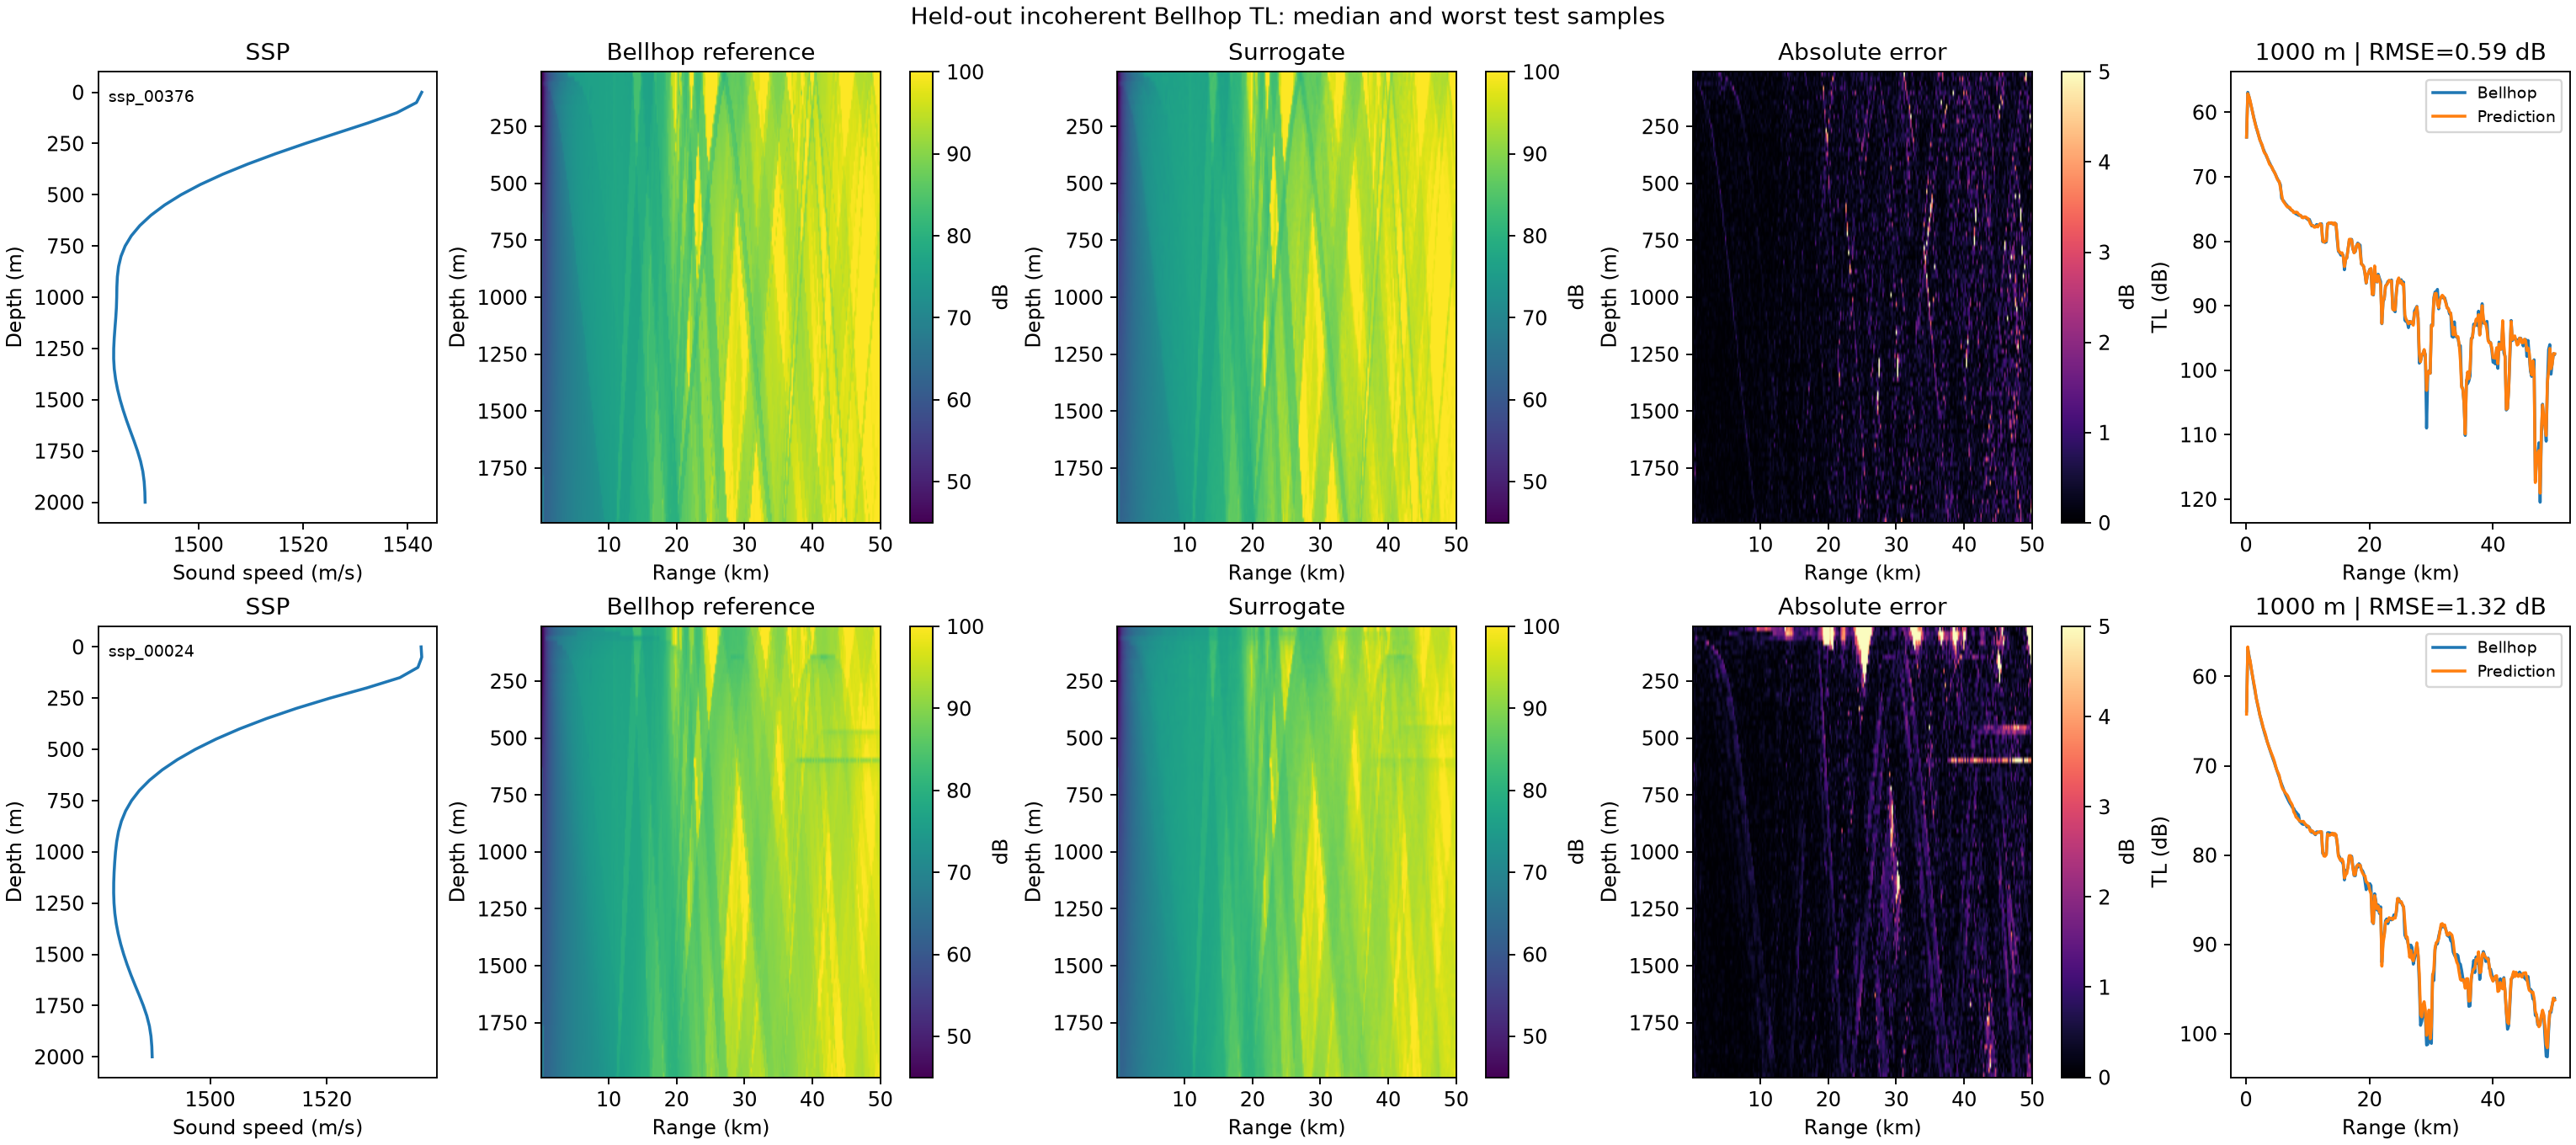
\includegraphics[width=\textwidth]{best_prediction_examples.png}
\caption{冻结测试集的中位样本（上）和最差样本（下）：SSP、Bellhop、代理预测、绝对误差与 1000 m 切片。}
\label{fig:examples}
\end{figure}

\subsection{计算效率}

Bellhop 正式数据单场计算中位时间为 9.138 s，改进型 FNO 在 A100 上 P95 为 4.732 ms。
按完整 96$\times$256 输出场的观测墙钟时间估算：
\begin{equation}
  S\approx\frac{9138\ \mathrm{ms}}{4.732\ \mathrm{ms}}\approx 1931.
\end{equation}
即代理模型的在线推理速度约为 Bellhop 的 1900 倍。这里比较的是项目实际使用的不同计算
后端上的端到端观测时间，其意义在于说明在线业务中的实际加速量级，而非宣称两种算法在
相同硬件上的理论复杂度比。

% -----------------------------------------------------------------------------
\section{结果讨论}

\subsection{为什么小数据集能够达到高精度}

512 条数据并不算大，但本任务中的频率、源深、水深、海底、输出网格和环境形态均被冻结，
SSP 变化又由四个平滑参数控制。因此学习问题的实际自由度远小于一般的跨海区、跨季节
声场预测。训练均值场 baseline 已达到 1.42 dB 也从侧面说明了这一点。FNO 的作用是进一步
利用 SSP 识别会聚位置和局部强度差异，把误差稳定压缩到约 0.52 dB。

\subsection{方法改进的作用}

实验表明，标准 FNO 已能完成核心映射；各向异性谱容量、非周期填充和残差连接则进一步
改善边界与会聚结构的拟合。均值场残差学习把固定几何下的共同 TL 趋势从学习目标中分离，
使有限模型容量更集中地表示 SSP 所引起的变化。最终方法的在线输入仅需要 SSP 与空间坐标，
不依赖额外环境特征或复杂的多任务损失，因此部署流程仍然简单。

\subsection{本报告结论的适用范围}

本报告的结果对应表~\ref{tab:task}定义的核心场景以及式~\eqref{eq:ssp}定义的 6 月型窄 SSP
环境族。当前数据没有覆盖其他月份、不同源深、不同频率、起伏地形、距离相关 SSP、不同
海底介质或三维多方位传播。若后续任务参数发生变化，应针对新增维度补充 Bellhop 标签并
重新验证，而不应直接把本报告数值外推到新的环境域。

在甲方 Bellhop 配置可用后，建议首先选择少量相同 SSP 和完全一致的环境参数做同 case
对齐，确认射线角、波束类型、插值方式和无效网格定义一致，再决定是否需要重新生成标签。
这一步不会改变本文提出的方法结构，但能够保证代理模型学习的参考解与最终验收软件一致。

\subsection{非平坦海底扩展说明}

从工程能力上看，现有 Bellhop 后端已经支持由控制点定义的分段线性 bathymetry，模型输入
也可以增加海底深度 $D(r)$ 和有效水体 mask 两个通道，因此少量、低维、平滑坡地形在方法上
是可扩展的。

但地形变化会直接改变射线路径、底反射、阴影区和有效接收区域，现有平坦海底 TL 标签不能
作为坡地形监督信号复用。任何有物理意义的地形扩展都必须重新生成并验证 Bellhop 标签。
基于当前阶段不新增 Bellhop 计算的约束，本报告不将坡地形纳入当前数据集和实验结果，只
保留上述接口与可行性结论。

% -----------------------------------------------------------------------------
\section{结论}

本项目围绕 1 kHz、50 km、2000 m 深海固定场景，完成了从 SSP 数据设计、Bellhop 高质量
标签生成到改进型 FNO 训练与密封测试的完整研究。数据集以项目提供的南海东侧 6 月仿真
深海 SSP 为原型，通过四个物理可解释参数生成 512 条平滑剖面；25,600 射线标签经过逐级
收敛验证，最高两级平均差异仅 0.052 dB。

针对深度--距离声场的各向异性和非周期边界，模型采用各向异性 Fourier modes、复制填充、
层间残差连接及训练均值场残差学习。最终测试 RMSE 为 0.5165 dB、MAE 为 0.1802 dB，
最差单样本 RMSE 为 0.7687 dB；A100 P95 推理时间为 4.73 ms。结果说明，在明确限定的
核心场景内，改进型 FNO 可以在保持主要会聚结构的同时，将完整二维声场计算从秒级降低到
毫秒级，并显著满足 2 dB / 100 ms 的目标要求。

% -----------------------------------------------------------------------------
\appendix
\section{关键数据与模型配置}

\begin{longtable}{L{5.0cm}L{9.0cm}}
\toprule
配置项 & 数值 \\
\midrule
\endhead
数据集 & 512 场；384/64/64 train/validation/test \\
SSP 原型 & 项目提供的南海东侧 6 月仿真深海声道形态 \\
SSP 参数 & 全局偏移、温跃层幅度、声道轴平移、深层梯度 \\
Bellhop & 非相干 TL，25,600 rays/场 \\
接收网格 & 96 depths $\times$ 256 ranges \\
输入 & 标准化 SSP + 深度坐标 + 距离坐标 \\
输出 & 相对训练均值 TL 场的标准化残差 \\
FNO & 4 层，32 channels，16$\times$48 modes \\
边界处理 & replicate padding：depth 8，range 16 \\
优化器 & AdamW，learning rate $10^{-3}$，weight decay $10^{-5}$ \\
训练 & batch 16，最多 180 epochs，cosine scheduler \\
最终参数量 & 6,300,417 \\
测试 RMSE / MAE & 0.5165 / 0.1802 dB \\
A100 P95 & 4.73 ms \\
\bottomrule
\end{longtable}

\section{复现与后续开发指南}

本节面向在甲方机器上继续开发的学生，给出从环境安装到独立验收的完整路径。仓库已经提供
一键脚本 \texttt{scripts/reproduce\_mvp.sh}。脚本默认只检查环境和单元测试，不会自动启动
耗时的 Bellhop 数据生成；必须显式选择 \texttt{REPRO\_MODE=full} 才会从零生成标签。

\subsection{复现范围与两条路径}

复现工作分为两种。

\begin{enumerate}
  \item \textbf{冻结数据复现：}甲方机器预先放置封存的 \texttt{dataset.npz}，学生只重新
  训练最终模型、计算测试指标和推理时延。该路径不运行 Bellhop，适合首先验证 Python、
  PyTorch、GPU 和报告结果链路。
  \item \textbf{从零复现：}先验证 Julia/Bellhop 后端，再进行 8 场射线数收敛、断点生成
  512 场 reference、训练最终模型并独立复核。该路径会实际运行 Bellhop，适合甲方数值
  环境已经确认后的完整复现。
\end{enumerate}

两种路径最终调用同一套训练和测试代码。建议学生先完成冻结数据复现，再决定是否进行
从零标签生成。

\subsection{机器与软件要求}

\begin{table}[H]
\centering
\caption{复现机器建议配置}
\begin{tabularx}{\textwidth}{L{3.6cm}Y}
\toprule
项目 & 要求或建议 \\
\midrule
操作系统 & Linux、WSL2 或 macOS；原生 Windows 尚未验证 \\
Python & 3.11，由 \texttt{uv} 安装并使用 \texttt{uv.lock} 锁定依赖 \\
数值后端 & JuliaCall 管理的 Julia 1.12；UnderwaterAcoustics.jl 0.8.1；AcousticsToolbox.jl 0.8.0 \\
GPU & 训练建议使用 NVIDIA CUDA GPU；无 GPU 可运行检查和 CPU 复核，但耗时不同 \\
磁盘 & 建议至少预留 20 GB，用于 Python/Julia 环境、Bellhop cases、数据和模型 \\
网络 & 首次安装需要取得 Python wheels、Julia 运行时和 Julia packages；离线机器需提前打包缓存 \\
\bottomrule
\end{tabularx}
\end{table}

若需要严格对比本报告 4.73 ms 的时延，应使用 NVIDIA A100 或重新在甲方指定硬件上建立
独立时延基准。不同 CUDA、FFT 和 CPU 后端可能带来轻微数值差异，不影响按 2 dB / 100 ms
门槛重新验收。

\subsection{仓库布局与版本固定}

两个仓库必须放在同一父目录下，因为 surrogate 的锁文件以相邻路径引用数值后端仓库。
目录结构如下：

\begin{lstlisting}[style=repro,language=bash]
acoustic-work/
  ocean-acoustic-agent/
  ocean-acoustic-surrogate/
\end{lstlisting}

联网机器可以执行：

\begin{lstlisting}[style=repro,language=bash]
mkdir -p acoustic-work && cd acoustic-work
git clone https://github.com/xuangu-fang/ocean-acoustic-agent.git
git clone https://github.com/xuangu-fang/ocean-acoustic-surrogate.git

# Pin the numerical backend used by the frozen dataset.
git -C ocean-acoustic-agent checkout \
  f07e8ea9a4fcb7bc66b4f36050b60d41d0fd959f

# This tag contains the report and reproduction appendix.
git -C ocean-acoustic-surrogate checkout technical-report-v1.2
\end{lstlisting}

甲方机器如果不能访问 GitHub，应在联网机器导出两个仓库的 bundle 或压缩包，并保留
\texttt{.git}、\texttt{uv.lock}、\texttt{juliapkg.json} 和配置文件。不要只复制若干 Python
文件，否则无法确认数值后端版本和数据哈希。

\subsection{环境安装与 Bellhop 自检}

首先在数值后端仓库完成完整自检：

\begin{lstlisting}[style=repro,language=bash]
cd acoustic-work/ocean-acoustic-agent
uv python install 3.11
uv sync --locked --extra dev

# Loads pinned Julia packages and solves one minimal Bellhop case.
uv run python scripts/check_env.py
\end{lstlisting}

只有完整自检明确输出 \texttt{Bellhop-ready}，才能认为数据生成机器已经就绪。
快速参数 \texttt{--quick} 只检查 Julia 包能否加载，不能代替 Bellhop 求解测试。
随后检查代理项目：

\begin{lstlisting}[style=repro,language=bash]
cd ../ocean-acoustic-surrogate
uv sync --locked
REPRO_MODE=check bash scripts/reproduce_mvp.sh
\end{lstlisting}

该命令运行 Ruff 和项目单元测试，不生成任何新标签。

\subsection{大型数据目录约定}

代码、配置和轻量结果进入 Git；大型数据、Bellhop cases、checkpoint 和完整预测保存在
\texttt{OCEAN\_SURROGATE\_ROOT}：

\begin{lstlisting}[style=repro,language=bash]
export OCEAN_SURROGATE_ROOT=/mnt/data/xuangu-fang/ocean-acoustics/\
projects/ocean-acoustic-surrogate
mkdir -p "$OCEAN_SURROGATE_ROOT"
\end{lstlisting}

关键目录结构为：

\begin{lstlisting}[style=repro]
$OCEAN_SURROGATE_ROOT/
  datasets/scs_june_narrow_v0.1/
    pilot/convergence_report.json
    n512/dataset.npz
    n512/manifest.json
    n512/samples/ssp_*/sample.npz
    n512/bellhop_cases/
  runs/<timestamp>_r3_padding_residual/
    model.pt
    metrics.json
    history.json
    predictions.npz
    independent_verification_<device>.json
  campaigns/latest.json
\end{lstlisting}

冻结数据复现至少需要 \texttt{dataset.npz} 和 \texttt{manifest.json}。正式数据文件的
SHA-256 应为：

\begin{lstlisting}[style=repro,language=bash]
sha256sum "$OCEAN_SURROGATE_ROOT/datasets/\
scs_june_narrow_v0.1/n512/dataset.npz"
# 13f4246b86a2fff33f2e5d587c1443be47eb15b4ad3d5c413688464ed8c7281d
\end{lstlisting}

如果哈希不一致，应先确认文件传输和路径，不应直接继续比较逐点预测。

\subsection{一键运行}

\subsubsection{仅检查环境，不运行 Bellhop}

\begin{lstlisting}[style=repro,language=bash]
cd acoustic-work/ocean-acoustic-surrogate
export OCEAN_SURROGATE_ROOT=/mnt/data/xuangu-fang/ocean-acoustics/\
projects/ocean-acoustic-surrogate
REPRO_MODE=check bash scripts/reproduce_mvp.sh
\end{lstlisting}

\subsubsection{从冻结数据训练最终模型}

将封存数据放到约定的 \texttt{n512/dataset.npz} 后执行：

\begin{lstlisting}[style=repro,language=bash]
REPRO_MODE=train bash scripts/reproduce_mvp.sh
\end{lstlisting}

脚本只选择最终结构 \texttt{r3\_padding\_residual}，不会重新运行报告中未采用的其他实验；
训练完成后会自动找到新 run directory，并在密封测试集上重新加载、计算指标和计时。

\subsubsection{从零生成 reference 并训练}

\begin{lstlisting}[style=repro,language=bash]
REPRO_MODE=full bash scripts/reproduce_mvp.sh
\end{lstlisting}

完整模式依次执行：Bellhop 自检、8 场射线收敛、512 场 reference 生成、数据 profile、最终
模型训练和独立复核。样本以 \texttt{sample.npz + metadata.json} 为断点，任务中断后再次执行
同一命令会跳过完整样本，不必从头重算。

\subsubsection{只复核已有模型}

\begin{lstlisting}[style=repro,language=bash]
export REPRO_RUN_DIR="$OCEAN_SURROGATE_ROOT/runs/\
<timestamp>_r3_padding_residual"
REPRO_MODE=verify bash scripts/reproduce_mvp.sh
\end{lstlisting}

\subsection{不使用一键脚本时的等价命令}

为了便于定位问题，一键脚本对应的核心命令如下：

\begin{lstlisting}[style=repro,language=bash]
# 1. Eight-profile ray convergence audit.
uv run ocean-acoustic-surrogate pilot configs/mvp.yaml --samples 8

# 2. Generate or resume 512 Bellhop reference fields.
uv run ocean-acoustic-surrogate generate configs/mvp.yaml --samples 512

# 3. Summarize and hash the packaged dataset.
uv run ocean-acoustic-surrogate profile configs/mvp.yaml --samples 512

# 4. Train only the final model.
uv run ocean-acoustic-surrogate campaign \
  configs/mvp.yaml configs/campaign.yaml \
  --samples 512 --only r3_padding_residual

# 5. Reload one run and score only the sealed test split.
uv run ocean-acoustic-surrogate verify configs/mvp.yaml \
  "$REPRO_RUN_DIR" --samples 512 --device auto

# 6. Rebuild all report figures and the PDF.
bash scripts/build_technical_report.sh
\end{lstlisting}

\subsection{核心代码位置}

\begin{table}[H]
\centering
\caption{学生继续开发时的代码入口}
\begin{tabularx}{\textwidth}{L{5.2cm}Y}
\toprule
文件 & 职责 \\
\midrule
\texttt{configs/mvp.yaml} & 频率、距离、网格、海底、SSP 参数域、数据划分和验收指标 \\
\texttt{configs/campaign.yaml} & 最终 FNO 结构、训练超参数和模型选择配置 \\
\texttt{src/.../ssp.py} & Latin hypercube 采样和四参数 SSP 构造 \\
\texttt{src/.../dataset.py} & Bellhop task、收敛审计、断点生成、mask 和数据封装 \\
\texttt{src/.../features.py} & SSP 插值、输入张量和训练均值场残差变换 \\
\texttt{src/.../models/fno.py} & 谱卷积、非周期 padding、残差 block 和投影头 \\
\texttt{src/.../training.py} & 训练、验证选模、测试、时延和 checkpoint 保存 \\
\texttt{src/.../verification.py} & 新进程重载、数据哈希、密封测试和独立计时 \\
\texttt{scripts/reproduce\_mvp.sh} & 面向甲方机器的一键复现入口 \\
\bottomrule
\end{tabularx}
\end{table}

表中 \texttt{src/...} 代表 \texttt{src/ocean\_acoustic\_surrogate/}。学生修改场景参数时，应先
新建配置和 dataset ID，不要直接覆盖 \texttt{scs\_june\_narrow\_v0.1}，以保证冻结结果仍可复核。

\subsection{Bellhop reference 生成代码示例}

下面代码与正式数据生成器使用同一接口，展示一条 SSP 如何变成一个 Bellhop reference：

\begin{lstlisting}[style=repro,language=Python]
from pathlib import Path
import numpy as np
from ocean_acoustic_agent import run_simulation
from ocean_acoustic_surrogate.config import MVPConfig
from ocean_acoustic_surrogate.dataset import build_task
from ocean_acoustic_surrogate.ssp import build_ssp_records

config = MVPConfig.from_yaml("configs/mvp.yaml")
record = build_ssp_records(
    config.ssp_family, n_samples=1, seed=config.contract.seed
)[0]
task = build_task(
    config,
    record,
    num_rays=config.contract.reference_num_rays,
    task_id="reference_smoke_00000",
)
result = run_simulation(task)
if result.status == "failed" or result.tl_field is None:
    raise RuntimeError(result.error_message)

tl_db = np.asarray(result.tl_field["tl_db"], dtype=np.float32)
valid_mask = np.isfinite(tl_db)
np.savez_compressed(
    Path("reference_smoke.npz"),
    tl_db=np.where(valid_mask, tl_db, 120.0),
    valid_mask=valid_mask,
    ranges_m=result.tl_field["ranges_m"],
    depths_m=result.tl_field["depths_m"],
    ssp_depths_m=record.depths_m,
    ssp_speeds_mps=record.speeds_mps,
)
\end{lstlisting}

正式生成不要手工循环这段示例，而应调用 \texttt{generate} 命令；正式实现会额外保存 case、
运行时间、split、配置哈希和失败记录，并支持断点续跑。

\subsection{最终模型训练代码示例}

若学生需要在 notebook 或自己的调度器中调用训练入口，可以直接选择最终实验配置：

\begin{lstlisting}[style=repro,language=Python]
from pathlib import Path
from ocean_acoustic_surrogate.config import MVPConfig, load_campaign
from ocean_acoustic_surrogate.training import run_experiment

mvp = MVPConfig.from_yaml("configs/mvp.yaml")
campaign = load_campaign("configs/campaign.yaml")
experiment = next(
    item for item in campaign["experiments"]
    if item["id"] == "r3_padding_residual"
)
dataset = (
    mvp.dataset_root / "n512" / "dataset.npz"
)
run_dir = run_experiment(
    mvp,
    dataset,
    experiment,
    campaign["training_defaults"],
)
print(run_dir)
\end{lstlisting}

训练入口只用 train split 拟合均值场和残差尺度，用 validation split 选择最佳 epoch，最后才
计算 test 指标。不要把测试样本混入训练，也不要按单个网格随机拆分数据。

\subsection{reference 评分与独立复核代码}

训练结束后推荐从新 Python 进程调用公开复核函数，而不是读取训练进程内变量：

\begin{lstlisting}[style=repro,language=Python]
from pathlib import Path
from ocean_acoustic_surrogate.config import MVPConfig
from ocean_acoustic_surrogate.verification import verify_run

mvp = MVPConfig.from_yaml("configs/mvp.yaml")
dataset = mvp.dataset_root / "n512" / "dataset.npz"
run_dir = Path("/path/to/<timestamp>_r3_padding_residual")
report = verify_run(mvp, dataset, run_dir, device_name="auto")
print(report)
\end{lstlisting}

复核过程会重新计算 dataset SHA-256、重建 SSP 特征、加载模型权重、只选择冻结 test split、
重新计算 RMSE/MAE 并执行 batch=1 P95 时延测试。输出写入 run directory，文件名为
\path{independent_verification_<device>.json}。

\subsection{预期产物与通过判据}

一次完整复现至少应保留以下文件：
\begin{itemize}
  \item 数据：\texttt{dataset.npz}、\texttt{manifest.json}、\texttt{convergence\_report.json}；
  \item 模型：\texttt{model.pt}、\texttt{metrics.json}、\texttt{history.json}；
  \item 预测：\texttt{predictions.npz}；
  \item 独立验收：\texttt{independent\_verification\_<device>.json}；
  \item 版本信息：两个仓库的 Git SHA、Python/Torch/CUDA/Julia packages 版本和配置哈希。
\end{itemize}

在相同冻结数据和 A100 环境下，应得到接近 0.5165 dB 的测试 RMSE 和 4.73 ms 的 P95。
在其他硬件上不要求逐位一致，但必须重新报告硬件、RMSE、MAE 和 P95，并检查三项验收值：
\begin{equation}
  \RMSE\leq2\ \mathrm{dB},\qquad
  \mathrm{MAE}\leq2\ \mathrm{dB},\qquad
  \mathrm{P95}\leq100\ \mathrm{ms}.
\end{equation}

如果结果不一致，排查顺序应为：数据 SHA、两个仓库 Git SHA、\texttt{mvp.yaml} 配置哈希、
Bellhop field mode 与 rays、数据 split、模型配置、设备和 CUDA/FFT 后端。不要先通过修改测试
划分或扩大误差阈值来“修正”结果。

\section{参考资料}

\begin{enumerate}[label={[\arabic*]}]
  \item Z. Li et al., ``Fourier Neural Operator for Parametric Partial Differential Equations,'' ICLR, 2021.
  \item M. B. Porter, \textit{The BELLHOP Manual and User's Guide: Preliminary Draft}, 2011.
  \item F. B. Jensen, W. A. Kuperman, M. B. Porter, and H. Schmidt,
  \textit{Computational Ocean Acoustics}, 2nd ed., Springer, 2011.
\end{enumerate}

\vfill
\begin{center}
\color{gray}\small —— 报告结束 ——
\end{center}

\end{document}
